\documentclass[a4paper]{article}

\usepackage[utf8]{inputenc}
\usepackage[T1]{fontenc}
\usepackage[italian]{babel}

\usepackage[margin=4.2cm, top=1.5cm, bottom=2.5cm]{geometry}

\usepackage{siunitx}
\usepackage{amsmath}
\usepackage{amssymb}
\usepackage{xfrac}
\usepackage{esint}
\usepackage[hidelinks]{hyperref}
\usepackage{graphicx}
\usepackage[font={sf}]{caption}
\usepackage{pdflscape}
\usepackage{makecell}
\usepackage{float}
\usepackage{subfig}
\usepackage{wasysym}
\usepackage{booktabs}

\setlength{\marginparwidth}{95pt}
\let\oldmarginpar\marginpar
\renewcommand\marginpar[1]{\oldmarginpar{\scriptsize\sffamily #1}}
\newcommand*\de{\mathrm{d}}
\newcommand*\pdv[2]{\frac{\partial #1}{\partial #2}}
\newcommand*\dv[2]{\frac{\de #1}{\de #2}}
\DeclareMathOperator\Ei{Ei}
\newcommand*\is{\equiv}
\newcommand\cs{$^{\text{137}}\text{Cs}$}
\newcommand\co{$^{\text{60}}\text{Co}$}
\newcommand\na{$^{\text{22}}\text{Na}$}
\newcommand\am{$^{\text{241}}\text{Am}$}
\newcommand\sr{$^{\text{90}}\text{Sr}$}

\sisetup{%
separate-uncertainty=true,
multi-part-units=single,
exponent-product=\cdot}

\frenchspacing

\title{Relazione di laboratorio:\\
Esperienza 3. Diffusione di Rutherford}
\author{Andrea Marasciulli
\and Giacomo Petrillo
\and Roberto Ribatti}
\date{13 marzo -- 20 aprile 2018}

\begin{document}

\maketitle

\begin{abstract}
	Verifichiamo l'andamento della sezione d'urto differenziale Rutherford,
	misuriamo il rapporto tra gli Z di alluminio e oro,
	confrontiamo la perdita di energia delle particelle $\alpha$ con dati noti
	e proviamo l'esistenza del backscattering.
\end{abstract}

{\tableofcontents}

\newpage
\section{Introduzione}

\subsection{Obiettivo}

Verificare l'andamento della sezione d'urto differenziale Rutherford per angoli acuti,
verificare la presenza di backscattering,
studiare la perdita di energia,
verificare il rapporto delle cariche nucleari di oro e alluminio.


\subsection{Apparato}

\begin{figure}
	\centering
	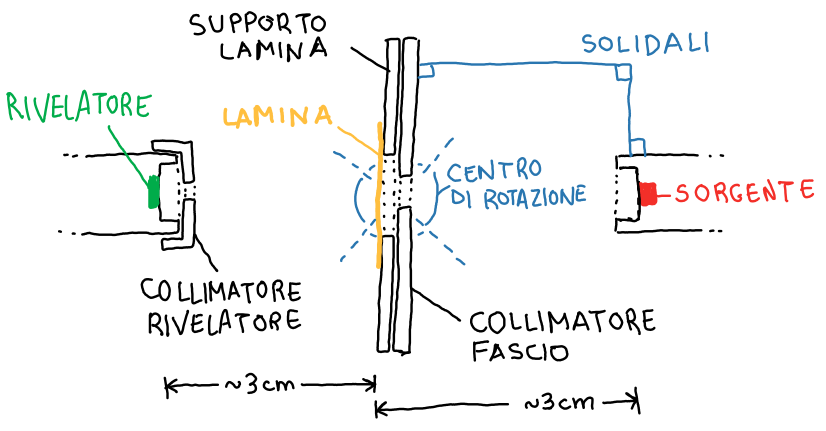
\includegraphics[width=28em]{immagini/schemacamera}
	\caption{\label{fig:schemacamera}
	Schema essenziale dell'apparato di misura.}
\end{figure}

La parte principale del nostro apparato è costituita da una camera a vuoto cilindrica con un diametro interno di  \SI{16.3(1)}{cm} e altezza \SI{8.4(1)}{cm} a cui è collegata la relativa pompa e i vacuometri.
\marginpar{ha senso scrivere l'errore su ste misure ? (Bob)}

Nel centro è possibile inserire un bersaglio che può essere ruotato solidalmente alla sorgente radioattiva $\alpha$
per variare l'angolo tra il proiettile e il rivelatore fisso, un fotodiodo al silicio (vedi \autoref{fig:schemacamera}).
La scheda dell'esperienza afferma che il rivelatore assorbe completamente le particelle $\alpha$,
permettendo di misurarne l'energia.

I bersagli a nostra disposizione sono lamine metalliche di diversi spessori:
\begin{itemize}
	\item oro: \SI{3}{\micro m}, \SI{5}{\micro m}, \SI{20}{\micro m} ($\times$2);
	\item alluminio: \SI{8}{\micro m} ($\times$2);
	\item acciaio: \SI{10}{\micro m};
	\item oro ``calibrato'': \SI2{\micro m};
	\item alluminio ``calibrato'': \SI8{\micro m}.
\end{itemize}
Le lamine ``calibrate'' sono quelle per le quali ci è garantito il valore dello spessore,
le altre lamine erano intese di prova.
Poiché abbiamo saputo solo alla fine dell'esperimento dell'esistenza di questa distinzione,
tutte le misure sono fatte con le lamine ``non calibrate'',
con le lamine ``calibrate'' abbiamo solo fatto delle misure di controllo.

I nostri proiettili sono le particelle $\alpha$ emesse da una sorgente di \am{} con attività \SI{330}{kBq} nel 1990 che si riduce a \SI{315}{kBq} nel 2018.
Possiamo scegliere di collimare il fascio incidente con due collimatori in plastica aventi una fessura rettangolare larga \SI{1}{mm} o \SI{5}{mm} ed altezza di \SI{5}{cm}.
La lamina bersaglio è in ogni caso accoppiata a una maschera circolare di diametro \SI{12}{mm}.
Il fotodiodo ha davanti a sé un collimatore rettangolare di dimensioni $2\times 6$\! mm rotabile a piacere.
\marginpar{spiegare in seguito che lo lasceremo sempre in verticale}

\paragraph{Elettronica di misura}

L'energia dei segnali del fotodiodo è misurata con un circuito preamplificatore-amplificatore-ADC.
Il circuito è triggerato da un discriminatore a soglia in tensione sul segnale del fotodiodo.
L'ADC è a 12 bit e fornisce anche il timestamp dell'evento con un round-time di 1.8 ore.
I segnali triggerati vengono anche contati da un modulo contatore.
Usiamo un timer in modalità bistabile per avviare e fermare contemporaneamente
il contatore e il circuito di misura dell'energia; il tempo è misurato dal conteggio \texttt{clock} del contatore. 


\section{Teoria}

\subsection{Sorgente}

La sorgente \am{} emette $\alpha$ a due energie cinetiche\footnote{PDG 2016 \S{} 37.}: \SI{5.443}{MeV}, \SI{5.486}{MeV}.
\marginpar{Oro attaccato alla sorgente fa calare l'energia.}
La sorgente emette anche raggi $\gamma$ a \SI{60}{keV} (\SI{36}\%),
per i quali la lunghezza di attenuazione nel silicio è circa\footnote{PDG 2016 fig. 33.18.}
$\SI{3}{g\,cm^{-2}} / \SI{2.6}{g\,cm^{-3}} = \SI{1.1}{cm}$.
Lo spessore del rivelatore è dell'ordine dei \si{\micro m}
e i fotoni vengono assorbiti con una probabilità circa del \SI{50}\%\footnote{NIST XCOM database \url{https://physics.nist.gov/PhysRefData/Xcom/html/xcom1.html}.},
allora la probabilità di assorbimento è circa \SI{1/20000}{\micro m^{-1}}.
Dalla scheda sappiamo l'area del fotodiodo (\SI{20}{mm^2})
e la distanza della sorgente dal fotodiodo ad angolo \SI0{\degree} è \SI{6}{cm},
quindi il rate atteso di fotoni che rilasciano tutta l'energia è
$\SI{315}{kBq} \times \SI{36}\% \times \SI{20}{mm^2} / (\SI{6}{cm})^2 \times \SI{1/20000}{\micro m^{-1}}
= \SI{0.03}{Hz\,\micro m^{-1}}$.
\marginpar{Ma quando vengono assorbiti i fotoni, poi vengono anche rivelati? Suppongo di sì.}

\subsection{Scattering Rutherford}

La sezione d'urto differenziale in approssimazione non relativistica di una particella di carica $+ze$ ed energia cinetica $T$ su un campo elettrostatico di carica $+Ze$ è\footnote{Wikipedia: Rutherford scattering \url{https://en.wikipedia.org/wiki/Rutherford_scattering}.}
\begin{equation}
	\label{eq:rutherford}
	\dv\sigma\Omega = \left( \frac {zZ\alpha\hbar c} {2T(1-\cos\theta)} \right)^2.
\end{equation}
Per un campo generato da una massa $M$ di carica $+Ze$,
applicando nella \eqref{eq:rutherford} le trasformazioni del problema in coordinate relative con la massa ridotta,
\marginpar{Mettere dimostrazione in appendice apposita.}
con $m$ massa della particella incidente e $T_\text{in}$, $T_\text{out}$ energia cinetica rispettivamente prima e dopo l'interazione, si ottiene
\begin{align*}
	T_\text{out}
	&= T_\text{in} \left( 1 - 2\frac mM(1-\cos\theta) + O\left(\frac mM\right)^2 \right), \\
	\dv\sigma\Omega &= \left( \frac {zZ\alpha\hbar c} {2T_\text{in}(1-\cos\theta)} \right)^2
	\left( 1 + O\left(\frac mM\right)^2 \right).
\end{align*}
Notiamo che la correzione al primo ordine nel rapporto delle masse alla sezione d'urto è nulla.

\subsection{Multiplo scattering}

Le particelle $\alpha$, passando nel bersaglio,
vengono in maggior parte deviate di piccoli angoli per interazione con molti atomi
e occasionalmente di un grande angolo per interazione con un singolo nucleo secondo la \eqref{eq:rutherford}.
Nel secondo caso comunque subiscono anche una deviazione ulteriore di un piccolo angolo
prima e dopo l'interazione ravvicinata con il nucleo.
La deviazione standard della distribuzione dei piccoli angoli,
nel limite non relativistico,
con l'angolo riferito a un piano fissato nello spazio anziché rispetto a un asse,
è data da\footnote{PDG 2016 \S{} 33.3.}
\begin{equation}
	\label{eq:ms}
	\theta_0 = \frac {\SI{6.8}{MeV}} {T_\text{in}} z \sqrt{\frac{x}{X_0}} \left(1+0.038\log\frac x{X_0}\right)
\end{equation}
dove $x$ è lo spessore attraversato e $X_0$ è la lunghezza di radiazione,
che vale\footnote{PDG 2016 \S{} 6.} \SI{8.9}{cm} per l'alluminio e \SI{0.33}{cm} per l'oro.
Ad esempio con $x = \SI5{\micro m}$ e $T_\text{in} = \SI5{MeV}$
risulta $\theta_0 = \SI{9}\degree$ per l'oro e \SI{1.5}{\degree} per l'alluminio.


\section{Misura e analisi}

\subsection{Strategia di acquisizione}

\paragraph{Angoli}
\label{spiegazione}
Ci accorgiamo che non siamo in grado di sistemare il coperchio della camera a vuoto esattamente nello stesso punto ogni volta che chiudiamo la camera. Eliminiamo questa sistematica sfruttando il fatto che il coperchio ha un foro che deve essere posizionato al di sopra di un perno. Dopo averlo incastrato lo spingiamo a sinistra e, una volta fatto il vuoto, la pressione atmosferica renderà impossibile spostarlo.
Questo accorgimento ci permette di riposizionare la sorgente nello stesso punto della scala graduata. Cercheremo gli angoli ``veri'' attraverso l'analisi delle nostre misure.
\marginpar{non so come spiegare questa cosa dell'angolo vero con parole migliori}
Riduciamo la parallasse nell'allineamento attaccando un pezzo di carta con una tacca al supporto della sorgente.
\marginpar{spiegare meglio il pezzo di carta (io metterei la foto senza aggiungere altro)}

\paragraph{Energia}
Per acquisire al meglio i segnali amplificati dobbiamo costruire un circuito che sincronizzi il contatore e l'ADC all'inizio e alla fine di ogni acquisizione.
Vogliamo comandare l'inizio e la fine di ogni acquisizione agendo sulla levetta di un timer.
I conteggi vengono effettuati collegando l'uscita TTL del discriminatore ad un generatore di impulsi non retriggerabile, la cui uscita va ad un contatore. Per far partire e fermare un'acquisizione elettronicamente è sufficiente collegare l'uscita del timer allo \emph{start} del contatore e l'\emph{end marker} allo \emph{stop}.
Per fare la stessa cosa con l'ADC colleghiamo l'uscita del timer (con durata impostata su $\infty$) ad un modulo di coincidenze a cui è connessa, ad un altro ingresso, l'uscita TTL del generatore di impulsi convertita in NIM. Il segnale di coincidenza (convertito in TTL) sarà il trigger dell'ADC, che deve arrivare all'omonimo ingresso \SI{1}{\micro s} prima del segnale affinché ne selezioni il picco.
Concludiamo la procedura inserendo i ritardi opportuni.

\paragraph{Precauzioni}
Evitiamo che segnali superiori a \SI{3.3}{V} danneggino l'ADC ponendo un attenuatore da \SI{0.9}{dB} all'uscita dell'amplificatore. Per il trigger non è necessario prendere precauzioni in quanto il convertitore NIM-TTL fornisce un segnale della tensione giusta. \marginpar{misurare?}

\paragraph{Salvataggio dati}
Il circuito descritto nel paragrafo \textbf{Energia} ha una particolarità: quando il crate si accende, il timer si riattiva e riavvia la catena di acquisizione.
Questo accorgimento è particolarmente utile se la corrente dovesse mancare mentre non siamo presenti. In tal caso l'ADC, al ritorno della corrente, registrerebbe i dati nella memoria interna (essendo il computer spento) ed essi sono facilmente recuperabili dopo la riaccensione del computer.


\subsubsection{Taratura ADC}
L'ADC è stata tarata ponendo la sorgente a \SI{0}{\degree} e variando il ritardo sul trigger fino a massimizzare la lettura del segnale. Il risultato di tale misura è presente in \autoref{tara}. Abbiamo acquisito lo spettro a vari angoli e verificato che l'energia delle particelle $\alpha$ non dipendesse dall'angolo in assenza di bersaglio. 
\marginpar{il fit e la figura sono degli scalda posto per sapere come verrà in seguito}
Abbiamo fittato lo spettro a \SI{0}{\degree} con una Gaussiana lasciandone libera anche la normalizzazione.\\
Abbiamo ottenuto:
\begin{align*}
\mu &=3115\pm2 \\
\sigma &= 87\pm2 \\
N &=(1.18\pm0.02)\cdot10^5 \\
\chi^2 &=2313\pm15 \\
\text{dof} &=15 \\
\end{align*}
Il valore elevato del $\chi^2$ mostra chiaramente la non gaussianità del picco osservato.

\begin{figure}[h]
\centering
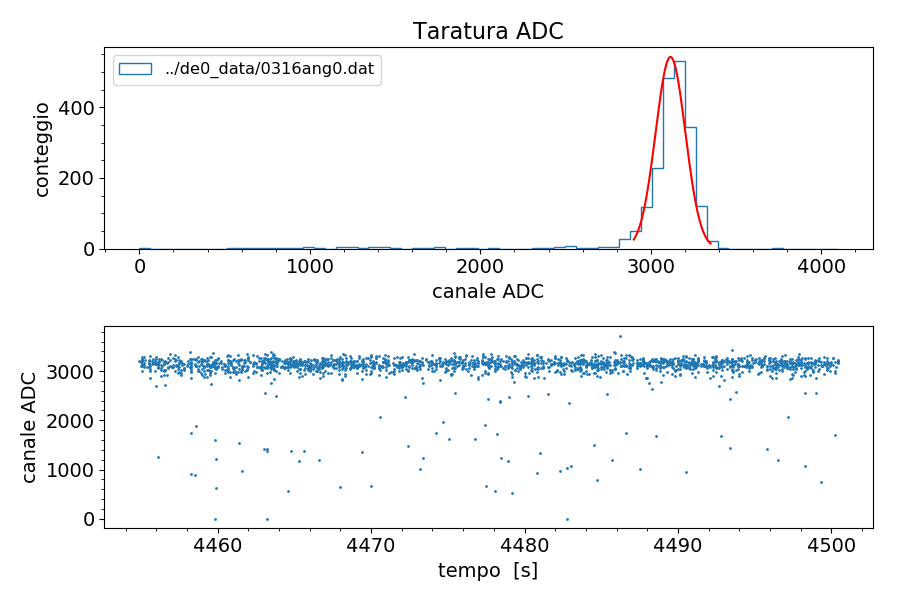
\includegraphics[width=23 em]{immagini/cal_provv}
\caption{Risoluzione in energia dell'ADC. Il pannello superiore mostra l'istogramma dei dati acquisiti con la funzione di fit, quello inferiore mostra il loro valore in funzione del tempo.}
\label{tara}
\end{figure}

\subsection{Pressione}

Variamo la pressione nella camera tenendo la sorgente a \SI{0}{\degree} per cercare in quali condizioni l'aria residua non influisce sulla misura.
Registriamo per ogni valore della pressione il rate di eventi ed il relativo spettro. In \autoref{tab:press} sono presenti i dati ed in \autoref{fig:press} il loro andamento.

\marginpar{qui mi riferisco agli angoli segnati sulla scala graduata, ricordiamoci che gli angoli rispetto al fotodiodo sono altri}

% tabella: angolo || rate || moda spettro (90)%CR -> spiegare quest'ultimo in caption
\marginpar{aggiungere la tabella}

\begin{figure}[h]
\centering
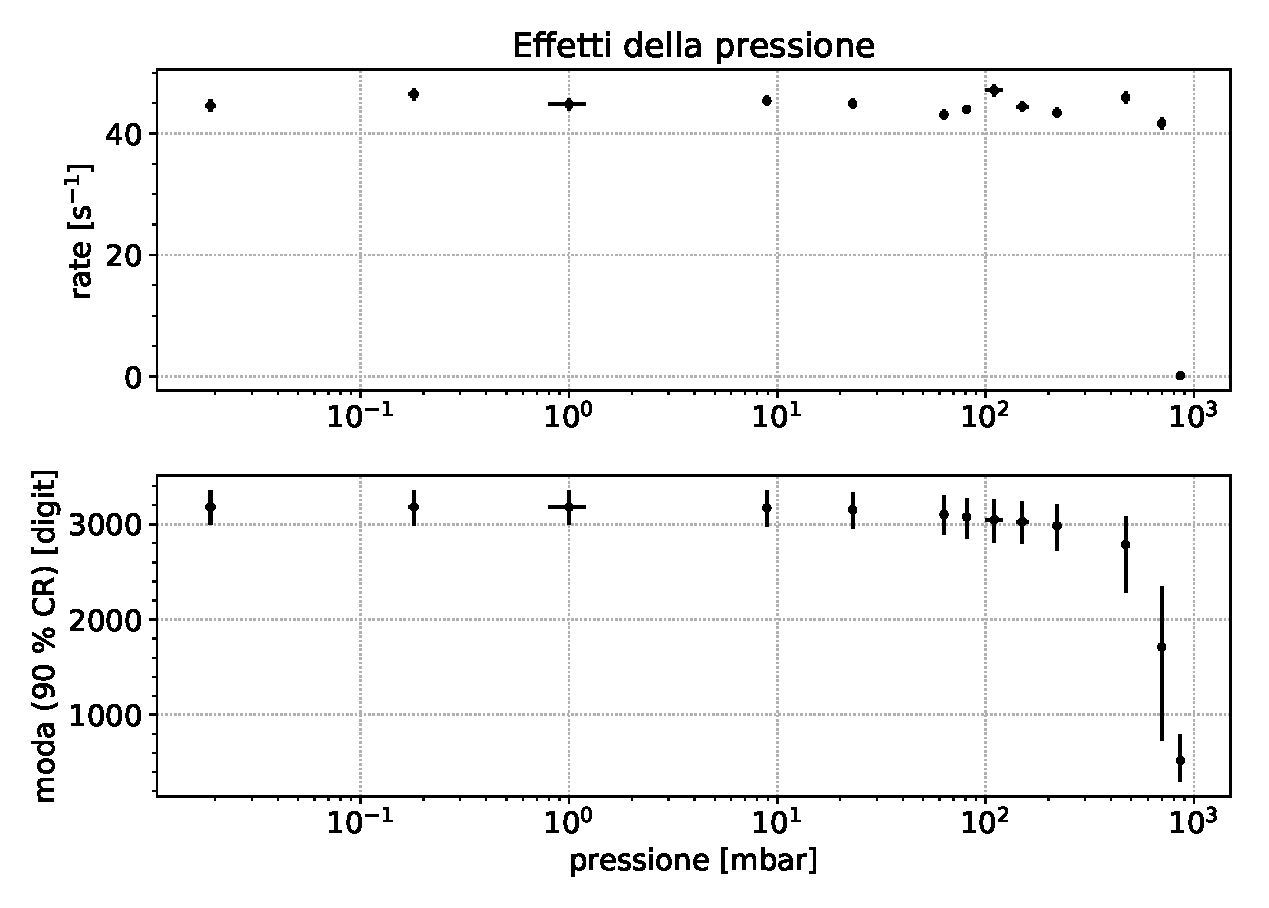
\includegraphics[width=30 em]{immagini/press}
\caption{Effetti della pressione su conteggi e spettri. Il pannello superiore mostra il variare del rate al variare la pressione, quello sottostante contiene la moda dei relativi spettri con errore un intervallo del 90\% di credibilità.}
\label{fig:press}
\end{figure}

\marginpar{Il 90\% di credibilità mi sembra eccessivo come errore. Si vedono i punti che scendono, ma gli errori enormi fanno credere che sia tutto compatibile. 
Ho guardato gli spettri e mi sono accorto che, alzando la pressione, le distro si allargano. Me ne farò una ragione.}

Dal grafico di \autoref{fig:press} non si nota nessuna variazione dei conteggi fino ad \SI{1}{atm}, ma la moda dello spettro inizia a decrescere quando la pressione è maggiore di \SI{200}{mbar}. 
Come atteso, la distribuzione di energia persa dalle particelle $\alpha$ in aria diventa sempre più larga all'aumentare della pressione.
Questo risultato ci assicura una grande indipendenza dalla condizione di vuoto della camera. 
\marginpar{aggiungere questione misure notturne}

\marginpar{secondo me dobbiamo mostrare questa cosa con l'istogramma di alcuni spettri perché dà un'idea più immediata rispetto al fornire l'intervallo di credibilità}

\subsection{Discriminatore}

\begin{figure}
	\hspace{-0.15\textwidth}
	{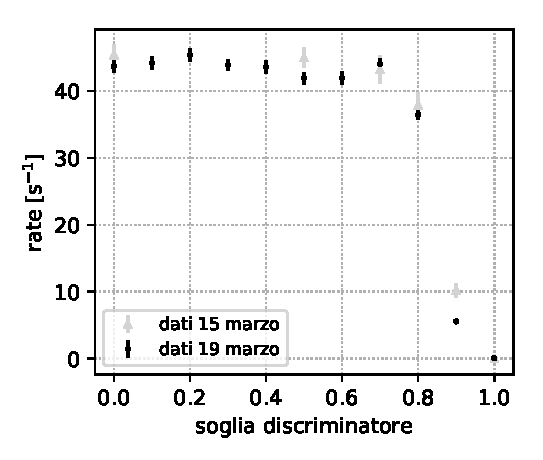
\includegraphics[width=0.6\textwidth]{immagini/soglia}}~
	{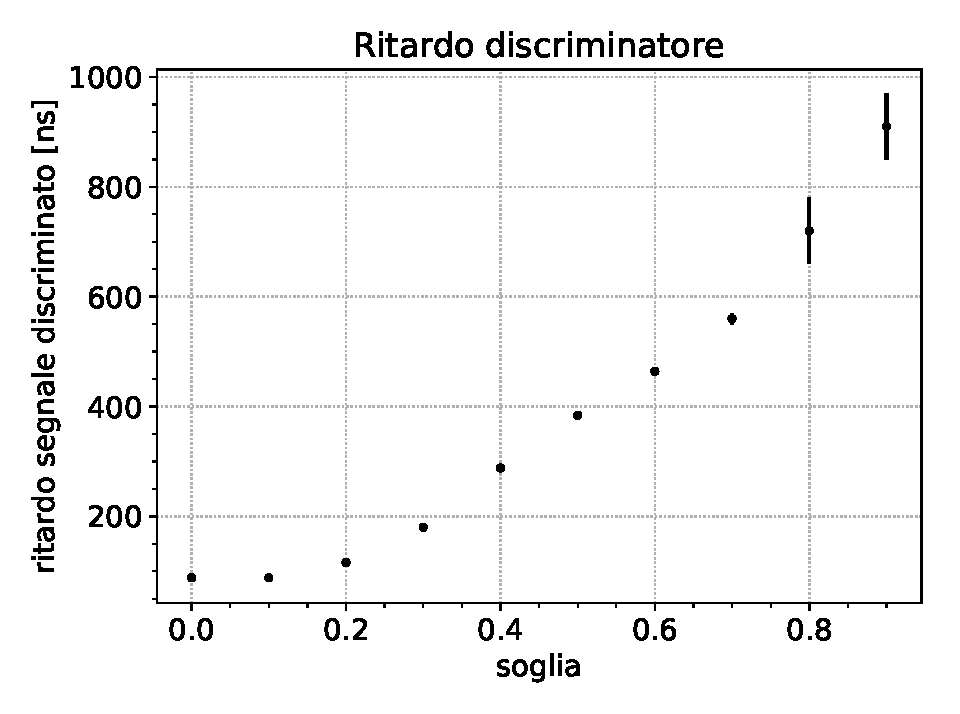
\includegraphics[width=0.6\textwidth]{immagini/ritardo}}
	\caption{\label{fig:sogliaritardo}
	Rate senza bersaglio al variare della soglia del discriminatore (sinistra)
	e ritardo temporale del segnale discriminato rispetto all'ingresso (destra).}
\end{figure}

La manopola di regolazione della soglia del discriminatore non indica l'unità di misura,
però con l'oscilloscopio vediamo che corrisponde circa ai volt quindi supponiamo siano proprio volt.

A \SI0{\degree} senza bersaglio misuriamo il rate al variare della soglia.
Poiché la soglia è in tensione e il segnale del fotodiodo è una curva a campana,
al variare dell'ampiezza del segnale o della soglia
cambia il ritardo del segnale discriminato rispetto a quello in ingresso,
quindi misuriamo anche il ritardo.
Le misure sono riportate in \autoref{fig:sogliaritardo}.
Dal fatto che il ritardo non cambi sulle due soglie più basse
stimiamo che la soglia minima effettiva sia circa \SI{100}{mV}.
Il ritardo introduce un bias verso il basso nelle misure di spettro,
ma non significativo rispetto alla larghezza degli spettri e ad altri problemi esposti di seguito.

% Variamo la soglia del discriminatore collegato al fotodiodo e registriamo il corrispondente rate di eventi a \SI0{\degree} senza collimatori.
% I valori di soglia riportati non hanno unità di misura perché sullo strumento sono solo presenti dei pallini e dei numeri interi.
% Non avendo trovato il manuale dello strumento, ci limitiamo a indicare la posizione del potenziometro.
% Scopriamo (\autoref{fig:soglia}) che il valore della soglia è ininfluente fino a 0.7 e si ha una repentina variazione dopo questo valore.
%
% Per sapere se la soglia ha un effetto minore di quanto misurato dobbiamo aumentare la statistica. I rates misurati hanno (nel migliore dei casi) una precisione del 2\%.
% Siccome il rate diminuisce di molto all'aumentare dell'angolo, le misure ad angoli maggiori avranno un'accuratezza minore. Quindi possiamo affermare che la soglia non avrà alcun effetto sulle misure di rate.
% Pertanto la teniamo a 0 per tutta l'esperienza.


\subsection{Forma del fascio}

Abbiamo fatto delle misure di conteggio a vari angoli con e senza collimatori per studiare la forma del fascio.

\subsubsection{Assenza di collimatori}

La misura in assenza di collimatori ci permette di indagare la forma del fascio di particelle $\alpha$ in uscita dalla sorgente di \am{}.
\marginpar{disegno provvisorio}
Bisogna notare che l'angolo segnato sulla scala graduata non coincide con quello tra la sorgente ed il rivelatore perché il fotodiodo non è al centro della camera a vuoto, inoltre all'aumentare (in modulo) dell'angolo la distanza tra sorgente e rivelatore diminuisce. 
Lo schema di \autoref{fma} illustra la situazione.

\begin{figure}[h]
\centering
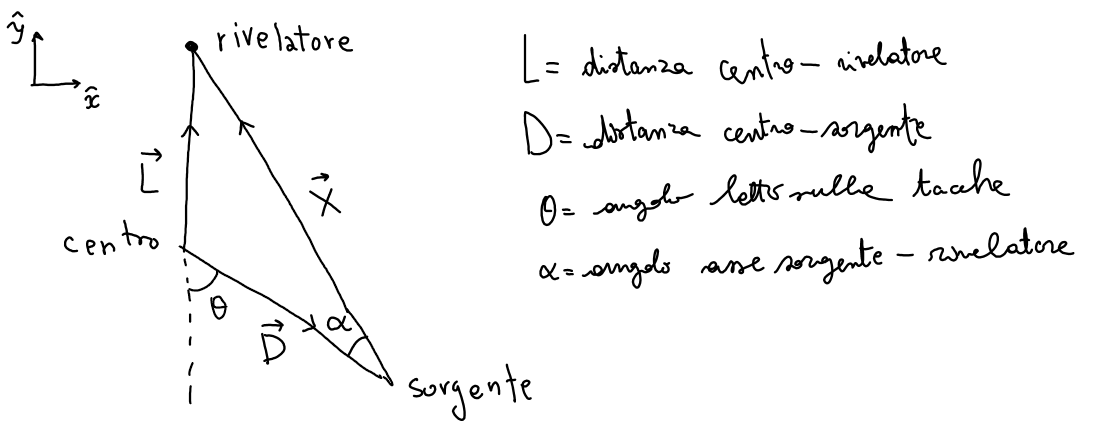
\includegraphics[width=30 em]{immagini/fma_provv}
\caption{Schema raffigurante gli angoli tra rivelatore, centro della camera a vuoto e sorgente.}
\label{fma}
\end{figure}

Applicate le dovute correzioni e usando le variabili di \autoref{fma} troviamo che l'angolo tra rivelatore e sorgente è
\begin{equation}
\cos{\alpha}= -\frac{\vec{X} \cdot \vec{D} }{ |\vec{X}| |\vec{D}| } = \frac{ L \cos{\theta} + D }{ \sqrt{ L^2+2LD\cos{\theta}+D^2  } }.
\end{equation}

Teniamo conto della variazione della distanza al variare dell'angolo moltiplicando ogni rate per $|\vec{X}|^2$.
Tale fattore è giustificato dal fatto che supponiamo isotropa l'emissione di particelle $\alpha$ da parte della sorgente.
Se $C$ è una costante, abbiamo che $$ \frac{dN}{d^3r}=C \implies \frac{dN}{dr}=C 4\pi r^2. $$

\marginpar{A dire il vero non lo so perché. Mi sembra che bisogna dividere per X$^2$ (analogia col campo elettrico). Invece moltiplichiamo. Il grafico ha senso ma non mi torna perché dovrei avere meno eventi all'allontanarmi dal rivelatore ad angolo fissato.}

Il risultato di questa misura è presente in \autoref{fig:form}, invece la \autoref{tab:form} contiene i dati di tale grafico.
Si evince che il fascio ha un'estensione angolare di quasi \SI{50}{\degree}.

\marginpar{inserire tante belle cose}

Useremo queste informazioni (se sarà necessario) nell'analizzare i dati sulla sezione d'urto.

\subsubsection{Collimatore da 5\! mm}

\subsubsection{Collimatore da 1\! mm}

\subsubsection{Collimatore a croce}

\subsection{Stabilità dell'ADC}

Facciamo una misura lunga circa 20 ore con la sorgente a \SI{70}{\degree} senza bersaglio per sapere ogni quanto l'ADC ha bisogno di essere ricalibrata. 
Abbiamo scelto questo angolo perché l'ADC ha un rate di campionamento massimo di \SI{40}{Hz}. In caso di rate maggiori salva gli eventi nella memoria interna finché non è piena; esaurita questa scrive sul file dei numeri casuali.
A \SI{70}{\degree} abbiamo un rate di circa \SI{35}{Hz}.

Mostriamo in \autoref{stab} i valori campionati dall'ADC in funzione del tempo. Non osserviamo nessuna variazione di energia rispetto ad una misura di breve durata.

\begin{figure}[h]
\centering
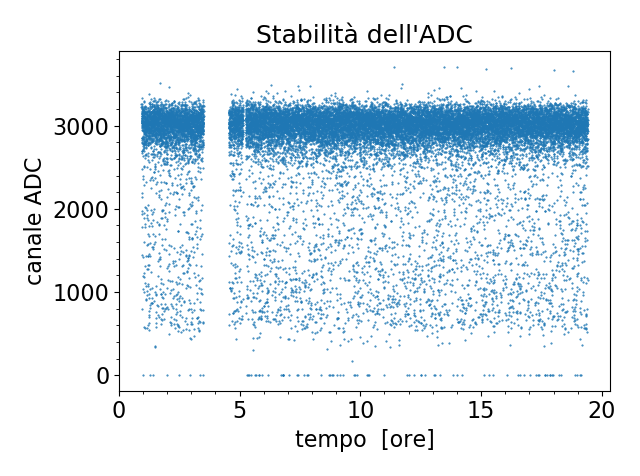
\includegraphics[width=30 em]{immagini/stab.png}
\caption{Valori acquisiti in funzione del tempo. Gli spazi vuoti tra una serie di dati e l'altra vengono dal fatto che sono state unite 4 acquisizioni quasi consecutive.
In questo grafico è presente soltanto un punto ogni 100 perché la rappresentazione completa rendeva illeggibile la figura.}
\label{stab}
\end{figure}

Guardando l'istogramma di questi dati ci siamo accorti che l'ADC presenta degli accumuli nei canali corrispondenti alle varie potenze di 2. Questo accade quando in un numero binario vengono cambiate più cifre alla volta, cosa che si verifica quando si raggiungono le varie potenze di 2. L'ADC impiega più tempo a cambiare valore e la misura successiva rimane nel bin precedente.
Per aggirare questo problema ribinniamo i dati usando dei bin che abbiano come bordi (0,32]+32n, dove n è un intero. Mostriamo questo effetto in \autoref{picchi} insieme alla sua ``correzione''.

\begin{figure}[h]
\centering
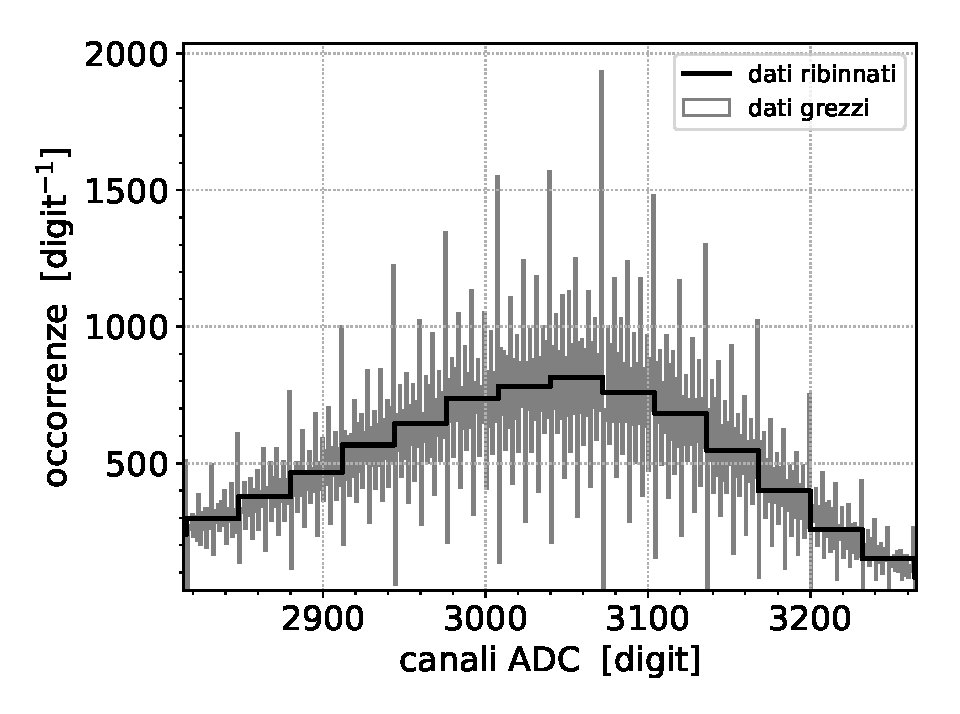
\includegraphics[width=30 em]{immagini/rebin}
\caption{Istogramma di una parte dei dati della misura di stabilità in cui si vedono gli accumuli a cui è soggetta l'ADC e la nostra soluzione.}
\label{picchi}
\end{figure}

\subsection{Misure}

Abbiamo eseguito le misure di rate al variare dell'angolo
con le lamine di oro da \SI{3}{\micro m} e \SI5{\micro m} e con quella di alluminio da \SI8{\micro m},
sia con il collimatore da \SI1{mm} che da \SI5{mm}.
In quasi tutte le misure abbiamo salvato lo spettro.




\subsection{Fit}

Misuriamo il rate di eventi al variare dell'angolo con i seguenti materiali:
\begin{itemize}
\item oro \SI{3}{\micro m}
\item oro \SI5{\micro m}
\item alluminio \SI8{\micro m}.
\end{itemize}




\subsubsection{Z dell'alluminio}

Comparando i parametri di ampiezza dei fit con l'oro con quello eseguito sull'alluminio, possiamo estrarre lo Z di quest'ultimo. Le ampiezze di fit hanno la forma $$ B=\mathcal{L} \left( \frac {zZ\alpha\hbar c} {2T} \right)^2 = \mathcal{L} A . $$
La nostra luminosità vale $\mathcal{L}=r n_2 l$, in cui $r$ è il rate di particelle incidenti, $n$  è la densità di bersagli e $l$ è lo spessore della targhetta.
Nel nostro caso $n_1$ è uguale per tutte le misure con lo stesso collimatore.   \marginpar{c'è bisogno di precisare perché?}
Da queste considerazioni possiamo trarre lo Z dell'alluminio dalla relazione \eqref{zeta} usando i parametri di fit per i dati con lo stesso collimatore.

\begin{equation}
Z_{\text{al}}=Z_{\text{au}} \sqrt{ \frac{B_{\text{al}}}{B_{\text{au}}} \frac{n_{\text{au}} l_{\text{au}}}{n_{\text{al}} l_{\text{al}}} }
\label{zeta}
\end{equation}

Otteniamo i seguenti risultati:

\begin{align*}
\text{Oro } \SI3{\micro m}&:\\
\text{collimatore } \SI1{mm}&: Z_{\text{al}}=\num{10.4(4)} \\
\text{collimatore } \SI5{mm}&: Z_{\text{al}}=\num{9.2(4)}. \\
\text{Oro } \SI5{\micro m}&:\\
\text{collimatore } \SI1{mm}&: Z_{\text{al}}=\num{13.5(6)} \\
\text{collimatore } \SI5{mm}&: Z_{\text{al}}=\num{70(2)}. \\
\end{align*}

Soltanto una misura è compatibile con lo $Z$ dell'alluminio atteso. Gli altri risultati sono influenzati dallo scattering multiplo all'interno dell'oro, fenomeno praticamente assente nell'alluminio.
L'ultimo risultato è molto lontano dal valore atteso perché lo scattering multiplo influisce pesantemente su una lamina d'oro così spessa e il fatto che il collimatore da \SI5{mm} selezioni più angoli rispetto a quello da \SI1{mm} non fa che peggiorare la situazione.

\subsection{Backscattering}

Poniamo le nostre lamine a \SI{150}{\degree} (il valore più grande sulla scala graduata) per verificare la presenza di backscattering. Usiamo 2 lamine attaccate per essere sicuri che nessuna particella attraversi il bersaglio. Questo accorgimento ci permette di evitare che delle particelle $\alpha$ entrino nel rivelatore dopo essere rimbalzate sulle pareti. Abbiamo controllato che questa ipotesi sia sensata contando le particelle che attraversano 2 lamine dello stesso materiale (e spessore) a \SI{0}{\degree}.

Facendo misure con \SI{40}{\micro m} di oro non abbiamo osservato nessun evento nei \SI{1406}s\,$\approx$\,\SI{23}{minuti} della misura. La situazione è diversa per \SI{16}{\micro m} di alluminio: abbiamo un rate di \SI{0.57(8)}{s^{-1}}.
Questo risultato però non è il nostro fondo perché nelle misure a \SI{150}{\degree} sarà rappresentato da quelle particelle $\alpha$ che, rimbalzando sulle pareti, arrivano nel fotodiodo. Sappiamo anche che il fondo maggiore è rappresentato dalle particelle che arrivano al rivelatore dopo aver rimbalzato sui supporti di plastica delle lamine.

Abbiamo quantificato quest'ultimo effetto ponendo un supporto senza lamina al centro della camera e misurando il rate a \SI{150}{\degree}. Otteniamo $R_{\text{buco}}=\SI{3.9(6)e-4}{s^{-1}}$.
Siccome in presenza dell'alluminio le particelle che raggiungono la parete opposta alla sorgente sono ancora meno che nella situazione precedente, possiamo affermare che il fondo è minore di quello misurato. Ci aspettiamo che il rate di fondo sia trascurabilmente minore di $R_{\text{buco}}$ sia per motivi geometrici che dinamici. La particella $\alpha$ in questione dovrebbe colpire un piccolo rivelatore rimbalzando in una grande camera a vuoto e la sezione d'urto differenziale Rutherford decresce molto velocemente per angoli inferiori a \SI{10}{\degree}. Inoltre, nei rimbalzi ad angolo maggiore, la perdita di energia è più elevata. Questi meccanismi sfavoriscono diffusioni multiple all'interno della camera.

Di seguito riportiamo i risultati delle nostre misure di backscattering:
\begin{align*}
R_{\text{oro}} &= \SI{1.3(2)e-3}{s^{-1}} \\
R_{\text{alluminio}} &= \SI{5.4(6)e-4}{s^{-1}} \\
R_{\text{fondo}} \simeq R_{\text{buco}} &= \SI{3.9(6)e-4}{s^{-1}} \\
\text{differenza oro-fondo} &= \SI{5.9(4)}{\sigma} \\
\text{differenza alluminio-fondo} &= \SI{2.6(11)}{\sigma} \\
\end{align*}

Possiamo affermare in modo indiscutibile l'esistenza del backscattering nel caso dell'oro, ma non possiamo fare altrettanto con l'alluminio, almeno in questa misura.
Per poter osservare un indiscutibile backscattering anche con l'alluminio, abbiamo posto 2 dissipatori di un pc in prossimità del fotodiodo e la sorgente a \SI{150}{\degree}.
\marginpar{inserire dimensioni dissipatori}
Le dimensioni dei dissipatori impediscono alle particelle $\alpha$ di attraversarli e sono colpiti dalla quasi totalità del fascio, restituendoci una misura praticamente priva di fondo.
L'autopassivazione dell'alluminio crea uno strato di ossido spesso da 1 a \SI5{nm}, che viene portato a 50--\SI{200}{nm} con processi industriali.%
\footnote{\url{http://www.valocchi.eu/logistica/alluminio.htm}}
Data la sottigliezza di tale spessore, consideriamo trascurabile la variazione del rate dovuta a questo strato e possiamo escludere che la presenza di ossigeno rilasciato nella camera possa interferire con la nostra misura.

\marginpar{Forse è meglio scrivere questa cosa all'inizio perché l'abbiamo trascurata anche per la lamina sottile.}

Abbiamo ottenuto \SI{54(7)}{eventi} in circa \SI{6.5}{ore}.

\appendix
\appendix
\section{Conti}
\label{sec:conti}

Calcoliamo la sezione d'urto Rutherford nel caso di nucleo non fisso.
La formula con nucleo fisso è
\begin{equation}
	\label{eq:ruthfisso}
	\dv\sigma\Omega = \left( \frac {zZ\alpha\hbar c} {2T(1-\cos\theta)} \right)^2.
\end{equation}
Il problema con il nucleo non fisso si rinconduce a quello fisso,
che chiamiamo <<problema ridotto>>, con queste sostituzioni:
\begin{center}
	\begin{tabular}{ll}
		Nucleo non fisso                 & Nucleo fisso               \\
		\hline
		Distanza tra particella e nucleo & Posizione della particella \\
		Massa della particella           & Massa ridotta              
	\end{tabular}
\end{center}
La \eqref{eq:ruthfisso} è da intendersi scritta nelle variabili del problema ridotto,
che dobbiamo esprimere in termini di quelle non ridotte.
Sia $\vec v$ la velocità della particella $\alpha$ (di massa $m$),
sia $\vec V$ la velocità del nucleo (di massa $M$), sia
\begin{equation*}
	\mu = \frac{mM}{m + M}
\end{equation*}
la massa ridotta.
Indichiamo con il pedice ``rid'' le variabili del problema ridotto.
La velocità ridotta è
\begin{equation*}
	\vec v_\text{rid} = \dv{}t(\vec r_\alpha - \vec r_\text{nucl}) = \vec v - \vec V.
\end{equation*}
Per conservazione dell'energia nel problema ridotto
$|\vec v_\text{rid,in}| = |\vec v_\text{rid,out}|$,
inoltre
$\vec v_\text{rid,in}
= \vec v_\text{in} - \vec V_\text{in}
= \vec v_\text{in}$.
Calcoliamo l'energia ridotta:
\begin{align*}
	\begin{cases}
		T_\text{rid} = \frac12 \mu v_\text{rid}^2 = \frac12 \mu v_\text{in}^2 \\
		T_\text{in}  = \frac12 m v_\text{in}^2
	\end{cases} \implies
	T_\text{rid} = \frac\mu m T_\text{in} = \frac1{1+\frac mM} T_\text{in},
\end{align*}
dunque abbiamo $T_\text{rid}(T_\text{in})$.
Ora ricaviamo $T_\text{out}$ in funzione di $T_\text{in}$ e $\cos\theta$.
Equivalentemente ricaviamo la relazione per le velocità anziché per le energie.
\begin{align*}
	\begin{cases}
		\vec v_\text{rid,out} = \vec v_\text{out} - \vec V_\text{out} \text{ (def. di $\vec v_\text{rid}$)}\\
		m \vec v_\text{in} = m \vec v_\text{out} + M \vec V_\text{out} \text{ (conservazione impulso)}
	\end{cases}
\end{align*}
ricaviamo $\vec V_\text{out}$ dalla seconda equazione:
\begin{align*}
	\vec V_\text{out} = \frac mM (\vec v_\text{in} - \vec v_\text{out})
\end{align*}
sostituiamo nella prima:
\begin{align}
	\label{eq:star}
	\vec v_\text{rid,out}
	= \vec v_\text{out} \left(1 + \frac mM\right) - \frac mM \vec v_\text{in}
\end{align}
prendiamo il modulo nell'ultima equazione:
\begin{align*}
	v_\text{in}^2
	= v_\text{out}^2 \left(1 + \frac mM\right)^2 + \left(\frac mM\right)^2 v_\text{in}^2
	- 2 \frac mM \left(1 + \frac mM\right) \vec v_\text{in} \vec v_\text{out}
\end{align*}
ma $\vec v_\text{in}\vec v_\text{out} = v_\text{in} v_\text{out} \cos\theta$.
Risolviamo per $v_\text{out}$:
\begin{align*}
	0
	&= v_\text{out}^2 \left(1 + \frac mM\right)^2
	- v_\text{out} 2\frac mM\left(1 + \frac mM\right) v_\text{in} \cos\theta
	- v_\text{in}^2 \left(1 - \left(\frac mM\right)^2 \right) = \\
	&= \left(1 + \frac mM\right) \Bigg(
   v_\text{out}^2 \left(1 + \frac mM\right)
  	- v_\text{out} 2\frac mM v_\text{in} \cos\theta
  	- v_\text{in}^2 \left(1 - \frac mM\right)
	\Bigg) \implies \\
	\implies v_\text{out}
	&= v_\text{in} \frac
	{\frac mM \cos\theta + \sqrt{\left(\frac mM\right)^2 \cos^2\theta + \left(1-\frac mM\right)\left(1+\frac mM\right)}}
	{1 + \frac mM} = \\
	&= v_\text{in} \frac
	{\frac mM \cos\theta + \sqrt{1 - \left(\frac mM\right)^2 (1-\cos^2\theta)}}
	{1 + \frac mM} = \\
	&= v_\text{in} \frac
	{\sqrt{1 - \left(\frac mM\sin\theta\right)^2} + \frac mM\cos\theta}
	{1 + \frac mM}
\end{align*}
dunque abbiamo $v_\text{out}(\vec v_\text{in},\cos\theta)$.
Ora ricaviamo $\cos\theta_\text{rid}$ in funzione di $\cos\theta$.
Prendiamo la proiezione su $\vec v_\text{in}$ della \eqref{eq:star}:
\begin{align*}
	\cos\theta_\text{rid}
	&= \frac{v_\text{out}}{v_\text{in}} \cos\theta \left(1+\frac mM\right) - \frac mM = \\
	&= \left( \sqrt{1 - \left(\frac mM \sin\theta\right)^2} + \frac mM \cos\theta \right) \cos\theta - \frac mM.
\end{align*}



\section{Tabelle}

\begin{table}[h]
\centering
\begin{tabular}{c|c|c}

pressione [mbar] & rate [\si{s^{-1}}] & moda [digit] \\
\hline
$ 0.0190 \pm 0.0010 $ & $ 44.6 \pm 0.9 $ & $ 3183 $ \\ 
$ 0.180 \pm 0.010 $ & $ 46.4 \pm 1.0 $ & $ 3182 $ \\ 
$ 1.00 \pm 0.20 $ & $ 44.8 \pm 0.9 $ & $ 3181 $ \\ 
$ 8.90 \pm 0.10 $ & $ 45.4 \pm 0.8 $ & $ 3172 $ \\ 
$ 23.0 \pm 1.0 $ & $ 44.9 \pm 0.9 $ & $ 3153 $ \\ 
$ 63.0 \pm 1.0 $ & $ 43.1 \pm 0.8 $ & $ 3103 $ \\ 
$ 81.0 \pm 1.0 $ & $ 44.0 \pm 0.7 $ & $ 3078 $ \\ 
$ 110 \pm 10 $ & $ 47.1 \pm 1.0 $ & $ 3049 $ \\ 
$ 150 \pm 10 $ & $ 44.4 \pm 0.9 $ & $ 3027 $ \\ 
$ 220 \pm 10 $ & $ 43.4 \pm 0.8 $ & $ 2984 $ \\ 
$ 470 \pm 10 $ & $ 45.9 \pm 0.9 $ & $ 2787 $ \\ 
$ 700 \pm 10 $ & $ 41.7 \pm 0.9 $ & $ 1712 $ \\ 
$ 860 \pm 10 $ & $ 0.13 \pm 0.04 $ & $ 521 $ \\ 

\end{tabular}
\caption{Dati per stimare l'effetto della pressione sulle misure. L'errore sulla moda è dato dall'intervallo di credibilità del 90\% calcolato sul relativo istogramma.}
\label{tab:press}
\end{table}


\begin{table}[h]
\centering

\begin{tabular}{c|c}
soglia & rate [\si{s^{-1}}] \\
\hline
$ 0.0 $ & $ 45.4 \pm 1.5 $\\ 
$ 0.5 $ & $ 45.0 \pm 1.5 $\\ 
$ 0.7 $ & $ 43.2 \pm 2.1 $\\ 
$ 0.8 $ & $ 38 \pm 2 $\\ 
$ 0.9 $ & $ 10 \pm 1 $\\ 
$ 1.0 $ & $\;\; 0.05 \pm 0.05 $\\ 
\hline
$ 0.0 $ & $ 43.7 \pm 0.9 $\\ 
$ 0.1 $ & $ 44 \pm 1 $\\ 
$ 0.2 $ & $ 45 \pm 1 $\\ 
$ 0.3 $ & $ 43.9 \pm 0.8 $\\ 
$ 0.4 $ & $ 43.6 \pm 0.9 $\\ 
$ 0.5 $ & $ 41.9 \pm 0.9 $\\ 
$ 0.6 $ & $ 42.0 \pm 0.9 $\\ 
$ 0.7 $ & $ 44.0 \pm 0.9 $\\ 
$ 0.8 $ & $ 36.5 \pm 0.7 $\\ 
$ 0.9 $ & $ 5.6 \pm 0.2 $\\ 
$ 1.0 $ & $ 0.05 \pm 0.03 $\\ 

\end{tabular}

\caption{Valori presenti nel grafico di \autoref{fig:soglia}. La linea orizzontale divide quelli del 15 marzo (in alto) da quelli del 19 marzo (in basso).}
\label{tab:soglia}
\end{table}



\begin{table}[h]
\centering

\begin{tabular}{c|c @{\,$\pm$\,} l}
soglia & \multicolumn{2}{c}{ritardo [\si{ns}]} \\
\hline
$ 0.0 $ & $ 88 $ & $ 2 $\\ 
$ 0.1 $ & $ 88 $ & $ 2 $\\ 
$ 0.2 $ & $ 116 $ & $ 2 $\\ 
$ 0.3 $ & $ 180 $ & $ 2 $\\ 
$ 0.4 $ & $ 288 $ & $ 2 $\\ 
$ 0.5 $ & $ 384 $ & $ 2 $\\ 
$ 0.6 $ & $ 464 $ & $ 4 $\\ 
$ 0.7 $ & $ 560 $ & $ 10 $\\ 
$ 0.8 $ & $ 720 $ & $ 60 $\\ 
$ 0.9 $ & $ 910 $ & $ 60 $\\ 
\end{tabular}

\caption{Dati per la misura in cui si quantifica il ritardo del segnale discriminato in funzione della soglia del discriminatore.
Le ultime misure hanno un errore maggiore a causa del jitter del segnale.}
\label{tab:rit}
\end{table}


\begin{table}[h]
\hspace{-3em}
\begin{tabular}{c|c|c||c|c|c}
	angolo [\si{\degree}] & rate  [\si{s^{-1}cm^2}] & moda [digit] & angolo [\si{\degree}] & rate  [\si{s^{-1}cm^2}] & moda [digit] \\
	\hline
	$ -42.6 \pm 1.5 $ & $ 5.2 \pm 1.3 $ & $ 1256 $                & $ 7.2 \pm 0.5 $ & $ 1.59 \pm 0.09   \cdot 10^{3} $ & $ 3140 $ \\  
	$ -38.0 \pm 1.3 $ & $ 257 \pm 16 $ & $ 2993 $                 & $ 9.6 \pm 0.5 $ & $ 1.56 \pm 0.09   \cdot 10^{3} $ & $ 3137 $ \\ 
	$ -33.3 \pm 1.1 $ & $ 538 \pm 31 $ & $ 3048 $                 & $ 12.0 \pm 0.6 $ & $ 1.45 \pm 0.08  \cdot 10^{3} $ & $ 3130 $ \\ 
	$ -31.0 \pm 1.0 $ & $ 6.6 \pm 0.4   \cdot 10^{2} $ & $ 3070 $ & $ 14.4 \pm 0.6 $ & $ 1.49 \pm 0.08  \cdot 10^{3} $ & $ 3125 $ \\ 
	$ -28.6 \pm 1.0 $ & $ 8.1 \pm 0.5   \cdot 10^{2} $ & $ 3087 $ & $ 16.7 \pm 0.7 $ & $ 1.36 \pm 0.08  \cdot 10^{3} $ & $ 3114 $ \\ 
	$ -26.2 \pm 0.9 $ & $ 9.7 \pm 0.5   \cdot 10^{2} $ & $ 3105 $ & $ 19.1 \pm 0.7 $ & $ 1.32 \pm 0.07  \cdot 10^{3} $ & $ 3101 $ \\ 
	$ -23.9 \pm 0.8 $ & $ 1.01 \pm 0.06 \cdot 10^{3} $ & $ 3113 $ & $ 21.5 \pm 0.8 $ & $ 1.28 \pm 0.07  \cdot 10^{3} $ & $ 3095 $ \\ 
	$ -21.5 \pm 0.8 $ & $ 1.10 \pm 0.06 \cdot 10^{3} $ & $ 3119 $ & $ 23.9 \pm 0.8 $ & $ 1.23 \pm 0.07  \cdot 10^{3} $ & $ 3087 $ \\ 
	$ -19.1 \pm 0.7 $ & $ 1.22 \pm 0.07 \cdot 10^{3} $ & $ 3129 $ & $ 26.2 \pm 0.9 $ & $ 1.19 \pm 0.07  \cdot 10^{3} $ & $ 3066 $ \\ 
	$ -16.7 \pm 0.7 $ & $ 1.22 \pm 0.07 \cdot 10^{3} $ & $ 3135 $ & $ 28.6 \pm 1.0 $ & $ 1.04 \pm 0.06  \cdot 10^{3} $ & $ 3047 $ \\ 
	$ -14.4 \pm 0.6 $ & $ 1.37 \pm 0.08 \cdot 10^{3} $ & $ 3134 $ & $ 31.0 \pm 1.0 $ & $ 9.5 \pm 0.5    \cdot 10^{2} $ & $ 3022 $ \\ 
	$ -12.0 \pm 0.6 $ & $ 1.39 \pm 0.08 \cdot 10^{3} $ & $ 3142 $ & $ 33.3 \pm 1.1 $ & $ 8.2 \pm 0.5    \cdot 10^{2} $ & $ 3002 $ \\ 
	$ -9.6 \pm 0.5 $ & $ 1.43 \pm 0.08  \cdot 10^{3} $ & $ 3144 $ & $ 35.7 \pm 1.2 $ & $ 6.5 \pm 0.4    \cdot 10^{2} $ & $ 2966 $ \\ 
	$ -7.2 \pm 0.5 $ & $ 1.45 \pm 0.08  \cdot 10^{3} $ & $ 3147 $ & $ 38.0 \pm 1.3 $ & $ 531 \pm 30 $ & $ 2937 $ \\  
	$ -4.8 \pm 0.5 $ & $ 1.47 \pm 0.08  \cdot 10^{3} $ & $ 3145 $ & $ 40.3 \pm 1.4 $ & $ 374 \pm 21 $ & $ 2892 $ \\  
	$ -2.4 \pm 0.5 $ & $ 1.55 \pm 0.08  \cdot 10^{3} $ & $ 3148 $ & $ 42.6 \pm 1.5 $ & $ 237 \pm 14 $ & $ 2840 $ \\  
	$ 0.0 \pm 0.5 $ & $ 1.56 \pm 0.09   \cdot 10^{3} $ & $ 3149 $ & $ 44.9 \pm 1.6 $ & $ 94 \pm 6 $ & $ 2717 $ \\  
	$ 2.4 \pm 0.5 $ & $ 1.56 \pm 0.09   \cdot 10^{3} $ & $ 3145 $ & $ 47.1 \pm 1.8 $ & $ 2.6 \pm 0.9 $ & $ 964 $ \\  
	$ 4.8 \pm 0.5 $ & $ 1.66 \pm 0.09   \cdot 10^{3} $ & $ 3141 $ & $ 7.2 \pm 0.5 $ & $ 1.59 \pm 0.09   \cdot 10^{3} $ & $ 3140 $ \\ 
\end{tabular}

\caption{Dati utilizzati per trovare la forma del fascio. L'errore sulla moda è dato dal 90\% di credibilità del relativo istogramma.}
\label{tab:forma}
\end{table}


\begin{table}[h]
\centering

\begin{tabular}{c|c|c}
angolo [\si{\degree}] & rate  [\si{s^{-1}}] & moda [digit] \\
\hline
$ -15.00 $ & $ 0.0 \pm 0 $ & $ 0 $ \\ 
$ -10.00 $ & $ 2.76 \pm 0.18 $ & $ 3177 $ \\ 
$ -7.50 $ & $ 27.8 \pm 0.6 $ & $ 3183 $ \\ 
$ -5.00 $ & $ 42.4 \pm 0.9 $ & $ 3186 $ \\ 
$ -2.50 $ & $ 43.9 \pm 1.0 $ & $ 3181 $ \\ 
$ 0.00 $ & $ 44.4 \pm 0.9 $ & $ 3185 $ \\ 
$ 2.50 $ & $ 44.7 \pm 1.0 $ & $ 3187 $ \\ 
$ 5.00 $ & $ 47.1 \pm 1.0 $ & $ 3182 $ \\ 
$ 7.50 $ & $ 43.2 \pm 0.9 $ & $ 3180 $ \\ 
$ 10.00 $ & $ 15.6 \pm 0.4 $ & $ 3188 $ \\ 
$ 15.00 $ & $ 0.0 \pm 0 $ & $ 0 $ \\ 

\end{tabular}

\caption{Rate in funzione dell'angolo con il collimatore da 5\! mm.
		L'errore sugli angoli è stimato essere 1.25$^{\circ}$.}
\label{tab:coll5}
\end{table}




\begin{table}[h]
\centering

\begin{tabular}{c|c|c}
angolo [\si{\degree}] & rate  [\si{s^{-1}}] & moda [digit] \\
\hline
$ -2.50 $ & $ 0.08 \pm 0.04 $ & $ 3156 $ \\ 
$ -1.25 $ & $ 2.48 \pm 0.20 $ & $ 3171 $ \\ 
$ 0.00 $ & $ 14.63 \pm 0.32 $ & $ 3174 $ \\ 
$ 1.25 $ & $ 31.5 \pm 0.7 $ & $ 3178 $ \\ 
$ 2.50 $ & $ 34.8 \pm 0.8 $ & $ 3185 $ \\ 
$ 3.75 $ & $ 26.9 \pm 0.6 $ & $ 3184 $ \\ 
$ 5.00 $ & $ 12.70 \pm 0.31 $ & $ 3188 $ \\ 
$ 6.25 $ & $ 2.81 \pm 0.22 $ & $ 3193 $ \\ 
$ 7.50 $ & $ 0.11 \pm 0.04 $ & $ 3185 $ \\ 

\end{tabular}

\caption{Dati per le misure con il collimatore da 1\! mm.}
\label{tab:coll1}
\end{table}



\begin{table}
\centering

\begin{tabular}{c|c|c}
angolo [\si{\degree}] & rate  [\si{s^{-1}}] & moda [digit] \\
\hline
$ -2.50 $ & $ 0.27 \pm 0.04 $ & $ 3213 $ \\ 
$ -1.25 $ & $ 1.20 \pm 0.11 $ & $ 3198 $ \\ 
$ 0.00 $ & $ 2.36 \pm 0.15 $ & $ 3190 $ \\ 
$ 1.25 $ & $ 2.56 \pm 0.16 $ & $ 3187 $ \\ 
$ 2.50 $ & $ 2.41 \pm 0.15 $ & $ 3192 $ \\ 
$ 3.75 $ & $ 1.32 \pm 0.09 $ & $ 3187 $ \\ 
$ 5.00 $ & $ 0.32 \pm 0.05 $ & $ 3193 $ \\ 

\end{tabular}

\caption{Dati per le misure con il collimatore a croce.}
\label{tab:super}
\end{table}





\end{document}